\documentclass{beamer}
\usepackage{hyperref}
\usepackage[T1]{fontenc}
\usepackage{latexsym,amsmath,xcolor,multicol,booktabs,calligra}
\usepackage{graphicx,pstricks,listings,stackengine}
\usepackage{tikz}

\author{Kirill Zemlianskii}
\title{Phsysics4LLM reproducibility study}
\subtitle{Syntetic data \& Canon layer ablations}
\institute{}
\date{March 2026}
\usepackage{CNU}
\setbeamertemplate{headline}{}

% Suppress auto-generated ToC frames at each section
\AtBeginSection{}

\definecolor{deepblue}{rgb}{0,0,0.5}
\definecolor{deepred}{rgb}{0.6,0,0}
\definecolor{deepgreen}{rgb}{0,0.5,0}
\definecolor{halfgray}{gray}{0.55}
\definecolor{CNUblue}{HTML}{3434b4}


\begin{document}

% ------------------------------------------------------------------
% Slide 1 — Title
% ------------------------------------------------------------------
\begin{frame}
  \titlepage
\end{frame}


% ==================================================================
\section{Motivation}
% ==================================================================

% ------------------------------------------------------------------
% Slide 2 — The Architecture Zoo Problem
% ------------------------------------------------------------------
\begin{frame}{The Architecture Zoo Problem}
  \textbf{Transformer variants keep multiplying:}
  \begin{itemize}
    \item Attention: sliding-window, MLA (DeepSeek), gated attention, DSA
    \item Positional encoding: RoPE, NoPE, ALiBi
    \item Gating: gated MLP, SwiGLU, MoE
  \end{itemize}

  \vspace{0.6em}
  \textbf{Why can't we just compare them?}
  \begin{itemize}
    \item Each change requires full re-training from scratch
    \item Academic scale (1.3B / 100B tokens): seed variance $\geq 2$--$4\%$
          swamps architecture differences of $1$--$2\%$
    \item Result: architecture ablations are slow, noisy, and expensive
  \end{itemize}
\end{frame}


% ==================================================================
\section{Synthetic Data as a Solution}
% ==================================================================

% ------------------------------------------------------------------
% Slide 3 — The Synthetic Playground Idea
% ------------------------------------------------------------------
\begin{frame}{The Synthetic Playground}
  \begin{columns}[T]
    \column{0.55\textwidth}
      \textbf{Idea:} Decompose ``intelligence'' into atomic skills;
      design one controlled task per skill.

      \vspace{0.5em}
      \textbf{Advantages:}
      \begin{itemize}
        \item Infinite high-quality data, zero cost
        \item Controlled difficulty — no skill mixing
        \item Short context, no CoT leakage
        \item Cheap enough to run at small scale
      \end{itemize}

      \vspace{0.4em}
      \small Design criterion: mental reasoning only,
      no CoT, short contexts, real-world relevant.

    \column{0.42\textwidth}
      \begin{block}{Physics 4.1 Task Suite}
        \begin{tabular}{@{}ll@{}}
          \textbf{Depo} & Reasoning depth \\
          \textbf{Brevo} & Reasoning breadth \\
          Capo & Knowledge capacity \\
          Mano & Knowledge manipulation \\
          Lano & Language structure \\
        \end{tabular}
      \end{block}
  \end{columns}
\end{frame}


% ==================================================================
\section{Task Descriptions}
% ==================================================================

% ------------------------------------------------------------------
% Slide 4 — Task Depo
% ------------------------------------------------------------------
\begin{frame}{Task Depo — Reasoning Depth}
  \textbf{Setup:} $k$-hop traversal over a directed permutation graph.
  No Chain-of-Thought allowed. Each node label can span multiple tokens.

  \vspace{0.4em}
  \textbf{Format:}
  \[
    \texttt{<bos>}\ x_1\ y_1 \quad x_2\ y_2 \quad \cdots \quad
    \texttt{<query\_}k\texttt{>}\ q \;\to\; a
  \]
  Edges presented in \emph{random} order. Model must chain $k$ retrieval
  steps entirely in activations.

  \vspace{0.4em}
  \textbf{Why it's hard:}
  \begin{itemize}
    \item $\text{max}$ $k$ determines the difficulty of the task
    \item No intermediate output tokens — all reasoning happens in the forward pass
    \item Must resolve depth-$k$ pointer chains in a single pass
  \end{itemize}
\end{frame}

% ------------------------------------------------------------------
% Slide 5 — Task Brevo
% ------------------------------------------------------------------
\begin{frame}{Task Brevo — Reasoning Breadth}
  \textbf{Setup:} Recursive DAG traversal — given root $q$, output all
  reachable nodes in topological order. Node labels can span multiple tokens.

  \vspace{0.5em}
  \begin{itemize}
    \item Parallel fan-out: multiple reasoning threads must be held
          simultaneously
    \item Model must compute the full topological sort \emph{before}
          emitting the first output token
    \item Graph size: up to 110 nodes
  \end{itemize}
\end{frame}


% ==================================================================
\section{Canon Layers}
% ==================================================================

% ------------------------------------------------------------------
% Slide 6 — Canon Layer Design
% ------------------------------------------------------------------
\begin{frame}{Canon Layers — Design}
  \textbf{Motivation:} Standard attention uses the \emph{full} global
  mechanism just to copy information to a neighbouring token.

  \vspace{0.4em}
  \textbf{Solution:} Lightweight horizontal residual links across
  neighbouring tokens:
  \[
    h'_t = h_t + w_0 \odot h_t + w_1 \odot h_{t-1} + w_2 \odot h_{t-2}
           + w_3 \odot h_{t-3}
  \]
  Element-wise, trainable weights per layer.

  \vspace{0.4em}
  \textbf{Implementation:}
  \begin{itemize}
    \item Causal \texttt{conv1d} with kernel size 4 + explicit residual
    \item $<0.01\%$ extra parameters for a 1.3B model
  \end{itemize}
\end{frame}

% ------------------------------------------------------------------
% Slide 6b — Canon Layer Insertion Points
% ------------------------------------------------------------------
\begin{frame}{Canon Layers — Insertion Points}
  \begin{columns}[T]
    \column{0.48\textwidth}
      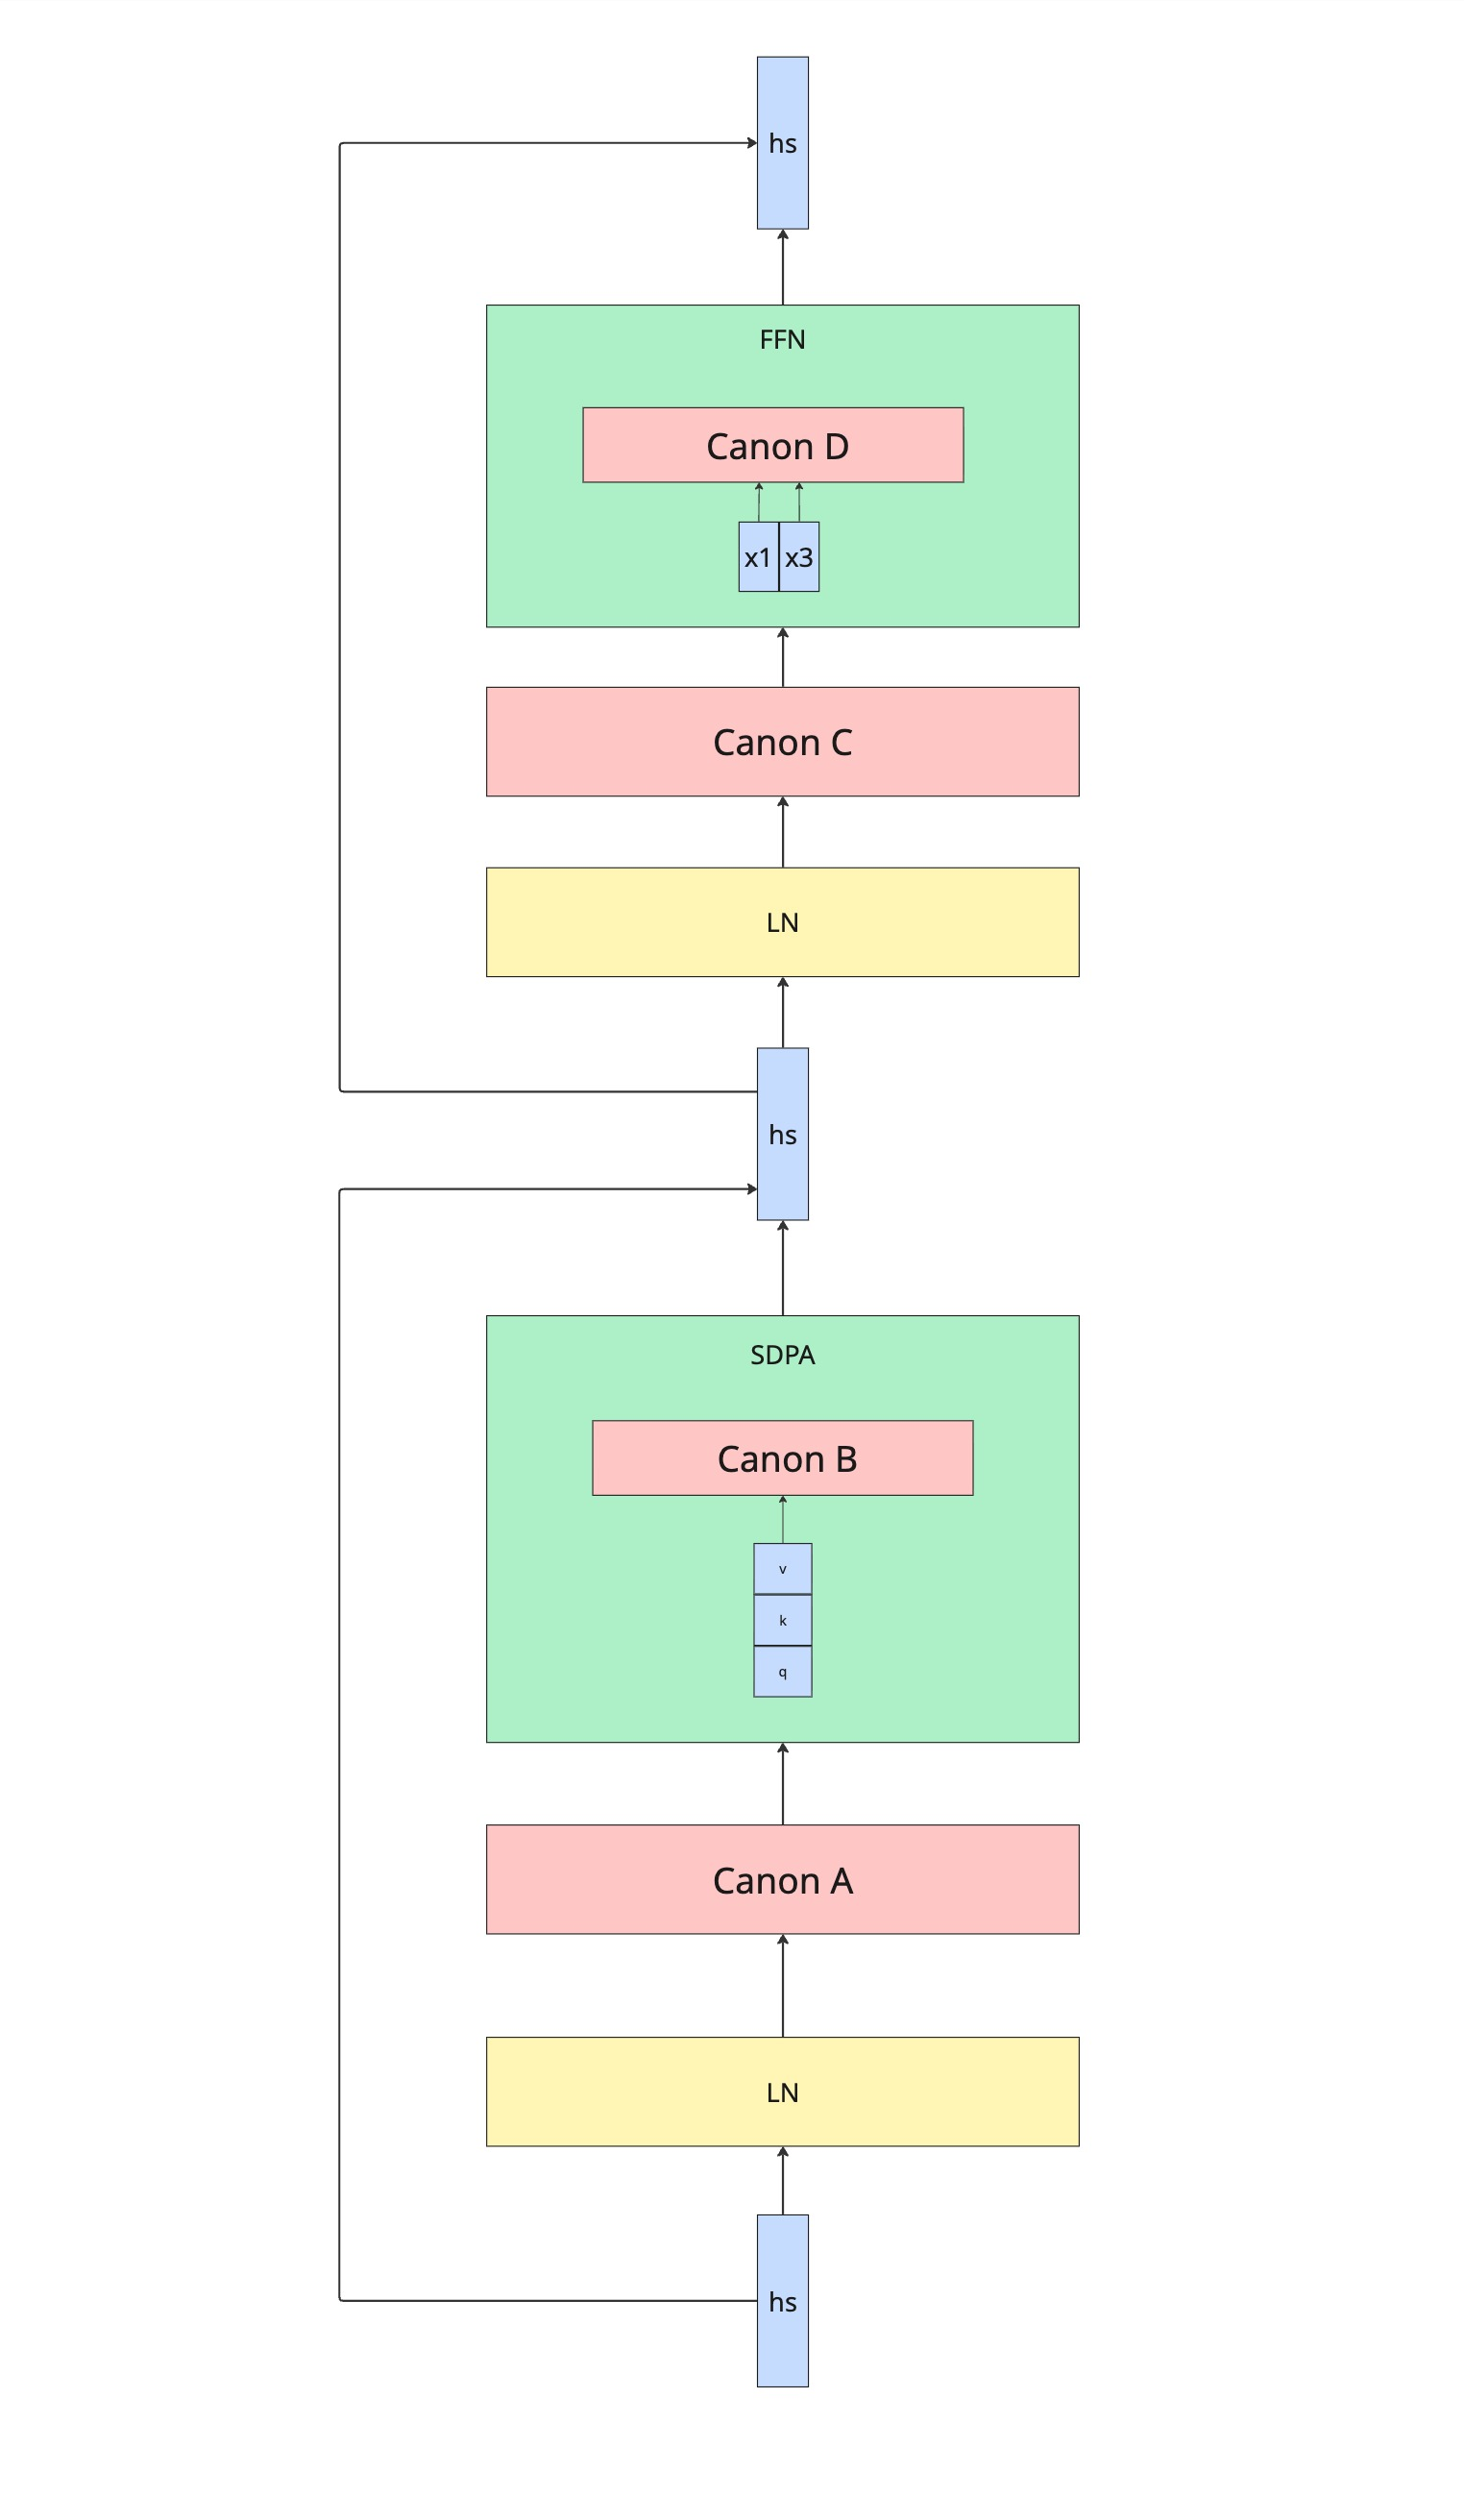
\includegraphics[width=\linewidth]{../plots/canon_location_scheme.jpg}

    \column{0.48\textwidth}
      \textbf{4 insertion points per transformer block:}
      \begin{itemize}
        \item[\textbf{A}] Pre-attention — before the attention sublayer
        \item[\textbf{B}] Q/K/V projections — inside attention, applied to query, key, and value
        \item[\textbf{C}] Pre-MLP — between attention output and the feed-forward sublayer
        \item[\textbf{D}] Inside MLP — between the two linear projections
      \end{itemize}
  \end{columns}
\end{frame}

% ------------------------------------------------------------------
% Slide 7 — Canon Results (paper claims)
% ------------------------------------------------------------------
\begin{frame}{Canon Results — Paper Claims}
  \textbf{Synthetic tasks (RoPE + Canon-ABCD):}
  \begin{itemize}
    \item Reasoning depth: $2$--$4\times$ improvement
    \item Reasoning breadth (Brevo): $+30\%$
    \item Knowledge manipulation (Mano): $+30\%$
  \end{itemize}

  \vspace{0.5em}
  \textbf{Architecture comparisons:}
  \begin{itemize}
    \item NoPE + Canon $\approx$ RoPE + Canon \quad (length generalisation)
    \item GLA + Canon $\approx$ Mamba2 / GDN \quad (simple baseline matches
          complex modern architectures)
    \item Real-world 1.3B / 100B tokens: Canon markedly improves NoPE and GLA
  \end{itemize}

  \vspace{0.4em}
  $\Rightarrow$ Synthetic task trends \textbf{mirror} real-world results.
\end{frame}


% ==================================================================
\section{Research Questions}
% ==================================================================

% ------------------------------------------------------------------
% Slide 8 — Research Questions
% ------------------------------------------------------------------
\begin{frame}{Research Questions}
  \begin{itemize}
    \item Can synthetic tasks be used to study training dynamics and the
          individual contribution of each architectural modification —

    \vspace{0.5em}
    \item Why does Canon help so much? Is it genuinely horizontal information
          mixing, or something else — like an implicit normalisation effect?

    \vspace{0.5em}
    \item How Canon parmeters impact performance?
          \begin{itemize}
            \item \textbf{Initialization} — does the starting magnitude of the
                  conv weights matter?
            \item \textbf{Kernel size} — how many past tokens should Canon look at?
            \item \textbf{Placement} — which layer depth and insertion point
                  (A/B/C/D) drives the gain?
          \end{itemize}
  \end{itemize}
\end{frame}


% ==================================================================
\section{Reproducibility}
% ==================================================================

% ------------------------------------------------------------------
% Slide 9 — Reproducibility Setup
% ------------------------------------------------------------------
\begin{frame}{Reproducibility Setup}
  \begin{columns}[T]
    \column{0.5\textwidth}
      \textbf{Framework:} Meta Lingua (\texttt{lingua\_modified})

      \vspace{0.5em}
      \textbf{Model:} Llama (RoPE), two sizes:
      \begin{itemize}
        \item 8 layers $\times$ 512 dim, 8 heads
        \item 12 layers $\times$ 768 dim, 12 heads
      \end{itemize}
      Tied input/output embeddings, \texttt{bf16}.

      \vspace{0.5em}
      \textbf{Training:} 100\,000 steps, AdamW,
      lr $3{\times}10^{-4}$, warmup 1\,000 — single A100

    \column{0.47\textwidth}
      \textbf{Tasks \& tokenization:}
      \begin{itemize}
        \item Depo / Brevo: pass-through tokenizer,\\
              batch 256, seq\,len 768
        \item Text: bytes tokenizer,\\
              batch 128, seq\,len 2048
      \end{itemize}

      \vspace{0.4em}
      \textbf{Loss:} cross-entropy\\
      (only on answer tokens for synthetic tasks)
  \end{columns}
\end{frame}


% ==================================================================
\section{Findings}
% ==================================================================

% ------------------------------------------------------------------
% Slide 10 — Findings summary
% ------------------------------------------------------------------
\begin{frame}{Findings}
  \begin{itemize}
    \item[\textbf{F1}] \textbf{Training is noisy.}
          Seed variance dominates convergence speed; use final accuracy over multiple seeds.

    \item[\textbf{F2}] \textbf{Default init is not optimal.}
          $w_0{=}1/k$ beats zero, default random, and baseline; wrong init recovers slowly.

    \item[\textbf{F3}] \textbf{First canon layer captures most of the benefit.}
          Last-layer Canon ≈ baseline; first-layer Canon ≈ full Canon-ABCD.

    \item[\textbf{F4}] \textbf{Consistent improvement with along with any norm placement.}
          Pre-LN has the fastest convergence and biggest boost from canon.

    \item[\textbf{F5}] \textbf{Larger kernel size improves convergence.}
          ks\,=\,6 $>$ 4 $>$ 2 $>$ baseline $>$ ks\,=\,1; kernel of 1 is worse than no Canon.

    \item[\textbf{F6}] \textbf{Canon mixes information \emph{and} normalises implicitly.}
          Higher weights on farther tokens; smoother gradients; fewer outlier activations.
  \end{itemize}
\end{frame}


% ==================================================================
\section{Discussion}
% ==================================================================

% ------------------------------------------------------------------
% Slide 16 — Discussion / Q\&A
% ------------------------------------------------------------------
\begin{frame}{Open Questions \& Future work}
  \begin{itemize}
    \item Training dynamics variance on synthetic data is determined by the task. What makes a task more noisy? How to design a task with training stability in mind?

    \vspace{0.4em}
    \item Is there a norm variation with training dynamics identical to canon.

    \vspace{0.4em}
    \item Reproduction with proper tokenizer.
  \end{itemize}
\end{frame}

% ------------------------------------------------------------------
% Slide 17 — Thank you
% ------------------------------------------------------------------
\begin{frame}
  \begin{center}
    {\Huge Thank you!}
  \end{center}
\end{frame}

\end{document}
